\documentclass[11pt,a4paper]{scrartcl}

%------------------------------------------%

\usepackage[utf8]{inputenc}
\usepackage[german]{babel}
\usepackage{amsmath}
\usepackage{amsfonts}
\usepackage{amssymb}
\usepackage{booktabs}
\usepackage{graphicx}
\usepackage{float}
%\usepackage{gnuplot-lua-tikz}
\usepackage{hyperref}
\usepackage{placeins}
\usepackage[bottom]{footmisc}
%------------------------------------------%


%------------------------------------------%
\newcommand{\Versuchsname}{Multivariate Data Analysis: \\ Higgs Challenge}			% Ändern!!
\newcommand{\Datum}{4. Februar 2015}			% Ändern!!
%------------------------------------------%


\begin{document}
%------------------------------------------%
%------------------------------------------%
\newcommand{\bra}[1]{\ensuremath{\left( #1 \right)}}
\newcommand{\abs}[1]{\ensuremath{\left| #1 \right|}}
\newcommand{\diff}[2]{\ensuremath{\frac{\partial #1}{\partial #2}}}

\newcommand{\HRule}{\rule{\linewidth}{0.5mm}}
\newcommand{\E}[1]{\textrm{#1}}
%------------------------------------------%
\begin{titlepage}
	\begin{flushright}
		
\includegraphics[width=0.4\textwidth]{kit_logo_de_farbe_positiv.jpg}\\[1cm]
	\end{flushright}
	\vspace{2cm}
	\begin{center}
	{\huge \textbf{Modern Methods in Data Analysis}}
	\vspace{1cm}

\HRule \\[0.4cm]
{ \huge \bfseries \Versuchsname}\\[0.2cm]
\HRule \\[0.5cm]

% Author and supervisor
\begin{flushleft}
	\begin{minipage}{0.4\textwidth}
	\large
		\begin{tabular}{l l}
			Lukas Fritz & 1686473 \\
			Fabian Leven & 1638446\\
			Ali Deniz Özdemir & 1724032\\
			Lena Salfenmoser & 1723697\\
			Johannes Heizmann & 1725035 \\
		\end{tabular}
	\end{minipage}
\end{flushleft}
\vfill

% Unterer Teil der Seite
{\large \Datum}
\end{center}

\end{titlepage}
\tableofcontents
\newpage
%------------------------------------------%




%------------------------------------------%
\numberwithin{equation}{section}

%------------------------------------------%

\section{Einleitung}
%\cite{bibtex.a}

Die ''Higgs-challenge'' wurde im Jahr 2014 von einer Gruppe von Wissenschaftlern der ATLAS-Kollaboration ins Leben gerufen. Dabei sollen die Originaldaten des ATLAS-Experiments auf Zerfälle des Higgs-Bosons in zwei Tau-Leptonen untersucht werden. Hierfür wurden Simulations- und Testdaten zur Verfügung gestellt, mithilfe derer Klassifikationsalgorithmen trainiert werden konnten, um schließlich im Original-Datenset zwischen ''Hintergrund'' und ''Tau-Tau-Zerfall eines Higgs'' unterscheiden zu können. Die ''challenge'' besteht dabei darin, die verschiedenen Methoden des maschinellen Lernens optimal auf die gegebene Situation anzupassen, sodass die Klassifizierung möglichst effizient erfolgen kann.

Das Training sowie die Analyse der Daten erfolgt mit dem ''Toolkit for Multivariate Data Analysis with ROOT'' (kurz: TMVA), das verschiedene Methoden des maschinellen Lernens bereitstellt. Von diesen waren vier (Maximum Likelihood-Methode, Fisher-Diskriminante, Boosted Decision Trees und neuronales Netzwerk) in einem Template vorgegeben. Die Mess- bzw. Trainingsdaten umfassten 30 Variablen. Da nicht alle gemessenen Werte eine Aussagekraft bezüglich der Entscheidung ''Hintergrund'' oder ''Signal'' besitzen, galt es zunächst, aus diesen 30 Variablen eine geeignete Untermenge auszuwählen. Anschließend wurde untersucht, inwiefern eine Transformation der (übrigen) Eingabevariablen, sowie eine Anpassung der Parameter der Algorithmen des maschinellen Lernens die Effizienz der Klassifizierung verbessern konnte. Ausschlaggebendes Kriterium war hierbei jeweils der im Training erzielte approximate median significance-Wert (kurz: AMS-Wert). Sobald ein zufriedenstellendes Ergebnis erreicht wurde, konnte der Klassifizierungsalgorithmus auf die Originaldaten angewandt werden.
\section{Getting familiar with the project}
\subsection{Correlation of Variables}
\begin{itemize}
\item determination of differences in correlations of signal and background
\item removal of non relevant variables
\end{itemize}
\subsection{Choosing a Classifier}
\section{improvement approach/Methodik}
\subsection{Improving the Classifier}
\subsection{Choosing the right cut}
\section{Fazit und unser Score}
Für die Analyse des kompletten Datensatzes verwendeten wir die BDT-Methode mit dem Parametersatz, der die besten Trainingswerte erreichte. (siehe Abschnitt \ref{sec:bdt_optimization}) Die Eingabevariablen wurden nicht transformiert und der volle Variablensatz wurde verwendet. Der erreichte AMS-Wert liegt bei
\begin{equation}
2.54
\end{equation}

\begin{figure}[htp]
\begin{center}
  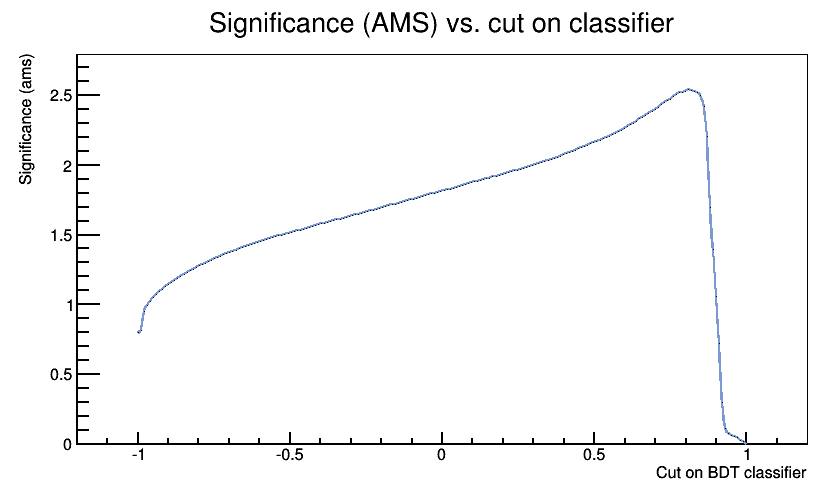
\includegraphics[width=0.7\linewidth]{sections/conclusion/AMS_vs_Cut_cropped.png}
 \caption[]{}
\label{fig:bdt_Shrinkage}
\end{center}
\end{figure}
%\bibliography{bibliography}
%\bibliographystyle{alpha}
%\bibliographystyle{unsrt}

\end{document}
